\section{Bias et Variance}

\begin{figure}[!h]
    \begin{minipage}{.40\linewidth}
        La notion entre bias et variance est importante, puisqu'il nous permet de prendre connaissance de la performance de notre système. Si on est en sous-apprentissage alors le bias est élevé, dans le cas d'un surapprentissage c'est la variance qui est élevée. De plus, à l'aide de c'est
        notions il est possible de déterminer la performance de notre système et de déduir le paramètre de régularisation optimal $\lambda$ \textit{cf \ref{sec:select-lambda}}.
    \end{minipage}\hfill
    \begin{minipage}{.56\linewidth}
        \begin{center}
            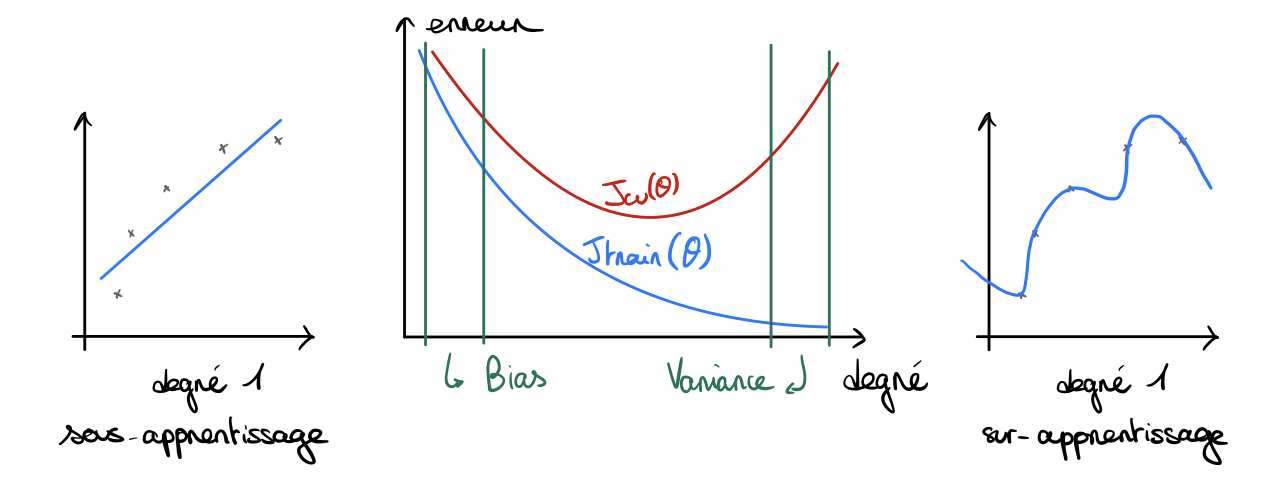
\includegraphics[width=1\textwidth]{./img/4.jpeg}
            \caption{\label{fig:bias-variance}Bias-Variance impacte}  
        \end{center}
    \end{minipage}
\end{figure}


\subsection{Courbe d'apprentissage}


La courbe d'apprentissage consiste à tracer l'erreur d'apprentissage et de validation en fonction de l'ensemble de données. \\
Pour ce faire, nous avons besoin de calculer c'est erreurs à l'aide du jeu de données et du jeu de validation. La fonction de coût nous permet d'obtenir l'erreur sur la prédiction, nous pouvons réutiliser cette fonction pour chaque nouvel échantillon.

\begin{figure}[!h]
\begin{minted}[frame=lines, framesep=2mm, baselinestretch=1.2, fontsize=\footnotesize, linenos, breaklines=true]{python}
def learningCurve(X, y, Xval, yval, Lambda):
    m, _ = X.shape
    error_train = np.zeros((m, 1))
    error_val = np.zeros((m, 1))

    for i in range(m):
        theta = trainLinearReg(X[:i+1,:], y[:i+1], Lambda)
        error_train[i], _ = linearRegCostFunction(X[:i+1,:], y[:i+1], theta, 0)
        error_val[i], _ = linearRegCostFunction(Xval, yval, theta, 0)

    return error_train, error_val

""" output
Training Examples   Train Error validation Error
    0       0.000000    205.121096
    1       0.000000    110.300407
    2       3.286595    45.010229
    3       2.842678    48.368911
    4       13.154049   35.865164
    5       19.443963   33.829961
    6       20.098522   31.970985
    7       18.172859   30.862446
    8       22.609405   31.135996
    9       23.261462   28.936206
    10      24.317250   29.551431
    11      22.373906   29.433816
"""
\end{minted}   
\captionof{listing}{\label{lst:learningCurve}Fonction learningCurve}
\end{figure}


\begin{figure}[!h]
    \begin{minipage}{.48\linewidth}
       Les erreurs obtenues nous permettent de tracer la courbe d'apprentissage. \\
       Nous pouvons observer que le bias est élevé, la courbe d'entrainement et de validation converge vers une erreur d'environ 25. Ce qui confirme notre hypothèse émit à la section 1.3, notre modèle est en sous-apprentissage dû aux faibles nombres de caractéristiques. \\

       Cette application nous permet également de comprendre l'importance de l'erreur de validation. Avec l'ensemble du jeu de donnée de validation, nous pouvons affiner nos paramètre pour optimiser nos 
       prédictions.
    \end{minipage}\hfill
    \begin{minipage}{.48\linewidth}
        \begin{center}
            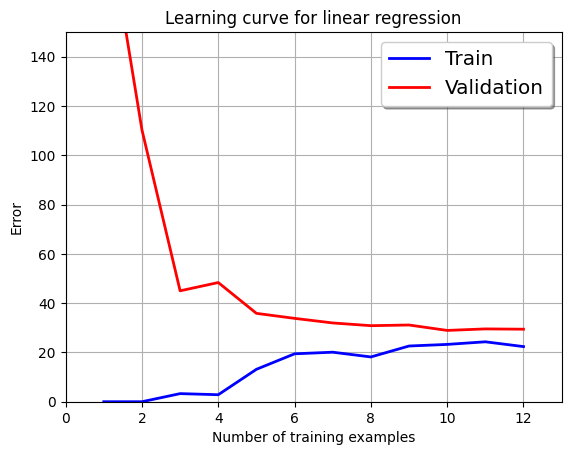
\includegraphics[width=0.9\textwidth]{./img/4.1.png}
            \caption{\label{fig:bias-variance}Courbe d'apprentissage}  
        \end{center}
    \end{minipage}
\end{figure}



